\documentclass[tikz,border=5pt]{standalone}
\usepackage[T1]{fontenc}
\usepackage{lmodern,amsmath,amssymb}
\usetikzlibrary{arrows.meta,calc,positioning,fit,backgrounds,shapes.geometric,matrix,decorations.pathreplacing,patterns}
\definecolor{ink}{gray}{0.08}
\definecolor{wash}{gray}{0.965}
\definecolor{soft}{gray}{0.45}
\tikzset{box/.style={draw=ink,line width=.65pt,fill=white,align=center,inner sep=4pt,outer sep=0pt,font=\small},flow/.style={draw=ink,line width=.65pt,-{Latex[length=1.8mm,width=1.3mm]},rounded corners=2pt},annotation/.style={font=\scriptsize,text=soft,align=center},groupbox/.style={draw=soft,dashed,line width=.45pt,fill=wash}}
\begin{document}
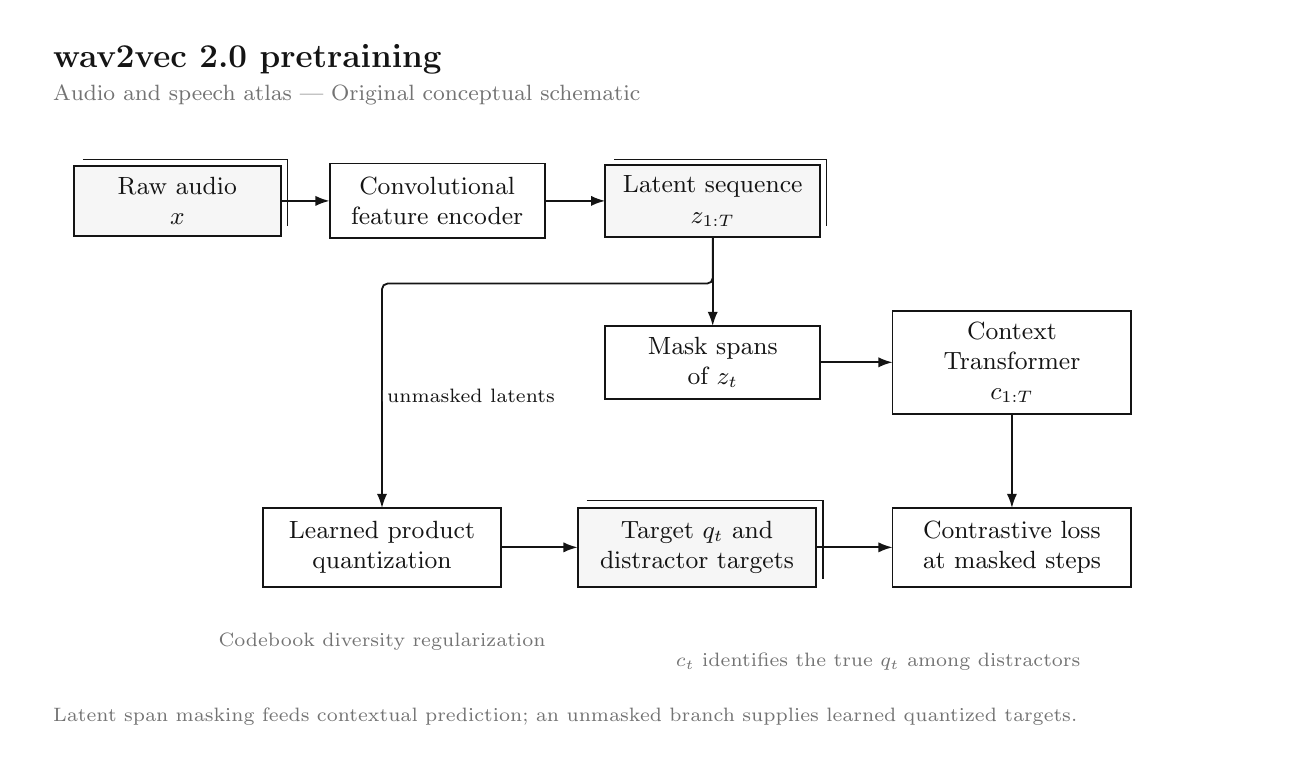
\begin{tikzpicture}[x=1cm,y=-1cm,font=\rmfamily,text=ink]

\path[use as bounding box] (0,0) rectangle (16,9);
\node[anchor=west,font=\large\bfseries] at (.2,.4) {wav2vec 2.0 pretraining};
\node[anchor=west,font=\footnotesize,text=soft] at (.2,.85) {Audio and speech atlas | Original conceptual schematic};
\begin{pgfonlayer}{background}
\end{pgfonlayer}
\node[box,fill=wash,minimum width=2.6cm,minimum height=0.85cm,text width=2.35cm] (wave) at (1.9,2.2) {Raw audio\\$x$};
\draw[ink,line width=.4pt] (0.6999999999999998,1.675) -- (3.3000000000000003,1.675) -- (3.3000000000000003,2.525);
\node[box,minimum width=2.7cm,minimum height=0.95cm,text width=2.45cm] (cnn) at (5.2,2.2) {Convolutional\\feature encoder};
\node[box,fill=wash,minimum width=2.7cm,minimum height=0.85cm,text width=2.45cm] (latent) at (8.7,2.2) {Latent sequence\\$z_{1:T}$};
\draw[ink,line width=.4pt] (7.449999999999999,1.675) -- (10.149999999999999,1.675) -- (10.149999999999999,2.525);
\node[box,minimum width=2.7cm,minimum height=0.85cm,text width=2.45cm] (mask) at (8.7,4.25) {Mask spans\\of $z_t$};
\node[box,minimum width=3.0cm,minimum height=0.95cm,text width=2.75cm] (context) at (12.5,4.25) {Context Transformer\\$c_{1:T}$};
\node[box,minimum width=3.0cm,minimum height=1.0cm,text width=2.75cm] (quant) at (4.5,6.6) {Learned product\\quantization};
\node[box,fill=wash,minimum width=3.0cm,minimum height=1.0cm,text width=2.75cm] (target) at (8.5,6.6) {Target $q_t$ and\\distractor targets};
\draw[ink,line width=.4pt] (7.1,6.0) -- (10.1,6.0) -- (10.1,7.0);
\node[box,minimum width=3.0cm,minimum height=1.0cm,text width=2.75cm] (loss) at (12.5,6.6) {Contrastive loss\\at masked steps};
\begin{pgfonlayer}{background}
\draw[flow] (wave.east) -- (cnn.west);
\draw[flow] (cnn.east) -- (latent.west);
\draw[flow] (latent.south) -- (mask.north);
\draw[flow] (mask.east) -- (context.west);
\draw[flow] (quant.east) -- (target.west);
\draw[flow] (target.east) -- (loss.west);
\draw[flow] (context.south) -- (loss.north);
\draw[flow] (latent.south) -- (8.7,3.25) -- (4.5,3.25) -- (quant.north) node[midway,right,fill=white,inner sep=1.5pt,font=\scriptsize] {unmasked latents};
\end{pgfonlayer}
\node[align=center,anchor=center,font=\scriptsize,text=soft,text width=5cm] at (4.5,7.8) {Codebook diversity regularization};
\node[align=center,anchor=center,font=\scriptsize,text=soft,text width=8cm] at (10.8,8.05) {\mbox{$c_t$} identifies the true \mbox{$q_t$} among distractors};
\node[anchor=west,align=left,font=\scriptsize,text=soft,text width=15.6cm] at (.2,8.75) {Latent span masking feeds contextual prediction; an unmasked branch supplies learned quantized targets.};
\end{tikzpicture}
\end{document}
